% Intestazione
\fancyhead[L]{4 \hspace{0.2cm} Pianificazione} % Testo a sinistra

% Sezione 
\section{Pianificazione}
\label{sec:pianificazione}
Il gruppo \emph{SWEg Labs} ha deciso di strutturare il proprio progetto in modo sistematico, 
organizzando le attività secondo scadenze ben definite, indicate all'inizio di ogni sezione. Le attività saranno suddivise in base alla fase di revisione e per argomento, garantendo così un approccio strutturato e focalizzato sui diversi stadi del progetto.\\
Un \emph{Diagramma di Burndown}\textsubscript{\textit{\textbf{G}}} fornirà una rappresentazione grafica dell'avanzamento del lavoro nel tempo, facilitando il monitoraggio costante del progresso e la gestione delle risorse.\\
Questo strumento consentirà al team di mantenere una visione d'insieme sull’avanzamento del progetto e di apportare eventuali aggiustamenti per rispettare le tempistiche pianificate.
Verrà redatto durante ogni \emph{sprint}\textsubscript{\textit{\textbf{G}}} un consuntivo dettagliato, che includerà sia i costi che le ore impiegate da ciascun membro del team. Tale analisi offrirà una chiara panoramica delle risorse investite e dei risultati ottenuti, rendendo possibile una valutazione complessiva 
dell’\emph{efficienza}\textsubscript{\textit{\textbf{G}}} e dell’\emph{efficacia}\textsubscript{\textit{\textbf{G}}} del progetto.
Il progetto del gruppo \emph{SWEg Labs} sarà suddiviso nelle seguenti fasi:
\begin{itemize}
    \item \textbf{Studio preliminare dei \emph{Capitolati}\textsubscript{\textit{\textbf{G}}}}: Analisi dei capitolati per valutare vantaggi e svantaggi di ciascuno, al fine di identificare quello che meglio si adatta alle competenze e agli interessi del gruppo, garantendo una scelta in linea con le esigenze progettuali. A seguire la candidatura per il capitolato scelto;
    \item \textbf{\emph{Requirements and Technology Baseline}}\textsubscript{\textit{\textbf{G}}}: Definizione dei requisiti e delle tecnologie di base necessarie per il progetto;
    \item \textbf{\emph{Product Baseline}}\textsubscript{\textit{\textbf{G}}}: Sviluppo del prodotto secondo i requisiti definiti.
\end{itemize}

Questa suddivisione consentirà al gruppo di avanzare in modo ordinato, 
assicurando che ogni fase del progetto sia completata in maniera ottimale per garantire il massimo livello di qualità e soddisfazione del cliente.

\vspace{0.5cm}

\subsection{Studio preliminare dei Capitolati}
\begin{table}[h!]
    \centering
    \renewcommand{\arraystretch}{1.5} % Aumenta l'altezza delle righe
    \begin{tabularx}{\textwidth}{|X|X|X|}\hline
    \rowcolor[HTML]{FFD700} 
    \textbf{Data di inizio} & \textbf{Data di fine} & \textbf{Aggiudicazione appalto} \\ \hline
    15/10/2024 & 31/10/2024 & 04/11/2024 \\ \hline
    \end{tabularx}
    \caption{Periodo dell’analisi dei Capitolati}
\end{table}

\subsubsection{Attività}
Il team \emph{SWEg Labs} ha condotto un’analisi approfondita dei capitolati proposti, valutandone con attenzione i vantaggi e gli svantaggi per individuare quello che meglio si adatta alle esigenze e alle competenze del gruppo. 
Questa analisi è fondamentale per l’elaborazione dell’\emph{Analisi dei Requisiti}\textsubscript{\textit{\textbf{G}}}, poiché la scelta del capitolato influenzerà in modo significativo la definizione dei requisiti di progetto.

\subsubsection{Periodo di sviluppo della candidatura}
Nella fase iniziale del progetto, il team \emph{SWEg Labs} si è concentrato su attività mirate a definire le linee guida fondamentali per assicurare un'esecuzione efficace e a stabilire i primi elementi identitari del gruppo.
Tra queste, verranno redatte le \emph{Norme di Progetto}\textsubscript{\textit{\textbf{G}}} e discussi i capitolati, offrendo ai membri l’opportunità di condividere preferenze e perplessità sulle varie proposte. Identificati i capitolati di maggiore interesse, il team avvierà contatti con i proponenti e organizzerà colloqui esplorativi per valutare le opzioni e preparare la candidatura.
In parallelo, saranno prese decisioni tecniche e logistiche come la scelta del nome del gruppo, la creazione del logo, la definizione di un indirizzo email di riferimento, la pianificazione delle riunioni e la selezione degli strumenti di comunicazione interni. Si avvierà anche la stesura del \emph{Glossario}\textsubscript{\textit{\textbf{G}}}, un elenco dei termini specifici utilizzati nei documenti per garantire chiarezza. Infine, saranno redatti verbali, sia interni che esterni, per registrare le decisioni prese e le attività da svolgere.
\newpage
\subsection{Requirements and Technology Baseline}
\begin{table}[h!]
    \centering
    \renewcommand{\arraystretch}{1.5} % Aumenta l'altezza delle righe
    \begin{tabularx}{\textwidth}{|X|X|}\hline
    \rowcolor[HTML]{FFD700} 
    \textbf{Data di inizio} & \textbf{Data di fine} \\ \hline
    04/11/2024 & 16/01/2025 \\ \hline
    \end{tabularx}
    \caption{Periodo dello sviluppo dell’RTB}
\end{table}
Il primo passo consiste nella definizione congiunta dei requisiti che il prodotto dovrà soddisfare durante il processo di sviluppo. In questa fase, il fornitore avrà la responsabilità di prendere decisioni chiave riguardanti le tecnologie, i framework e/o le librerie da utilizzare, al fine di assicurare l'adeguatezza e la fattibilità del progetto.
Successivamente, sarà fondamentale dimostrare la validità di tali scelte attraverso la realizzazione di un \emph{Proof of Concept}\textsubscript{\textit{\textbf{G}}}, conforme agli obiettivi stabiliti.
Le scelte tecnologiche e i dettagli di implementazione verranno documentati con attenzione.
Il codice e la documentazione saranno archiviati in due repository distinti: uno dedicato esclusivamente alla documentazione e un altro riservato al codice. Entrambi i repository saranno facilmente accessibili al proponente e ai committenti, costituendo punti di riferimento per monitorare l’avanzamento del progetto e garantendo completa trasparenza sulle decisioni e sulle attività svolte.

Le fasi principali della Requirements and Technology Baseline saranno suddivise come
segue:
\begin{itemize}
\item \textbf{Analisi e documentazione}: verrà condotta un’attenta analisi dei requisiti, basata sugli incontri con il proponente e sul capitolato, concentrandosi parallelamente sulla creazione e lo sviluppo della documentazione necessaria;
\item \textbf{Definizione delle tecnologie}: il fornitore selezionerà in modo ponderato le tecnologie da utilizzare, valutando criteri quali maturità, scalabilità e adattabilità alle esigenze specifiche del progetto;
\item \textbf{Sviluppo del {\emph{Proof of Concept}}}: la validità delle scelte effettuate verrà dimostrata tramite la realizzazione di un Proof of Concept, un prototipo funzionale che rispecchierà gli obiettivi stabiliti e fornirà un esempio concreto delle soluzioni e capacità proposte.
\end{itemize}

\subsubsection{Attività}

\begin{itemize}
\item \textbf{\emph{Norme di Progetto}}\textsubscript{\textit{\textbf{G}}}: Questo documento è fondamentale per definire con precisione tutte le regole che il team \emph{SWEg Labs} dovrà seguire durante lo sviluppo. Le norme forniscono un punto di riferimento per ogni membro del team, contribuendo a mantenere elevati livelli di coerenza e coesione. L'adozione di queste regole avrà un impatto significativo su ogni prodotto futuro, costituendo la base per le fasi successive. La definizione accurata delle norme è cruciale per garantire la qualità dei prodotti e l’allineamento con gli obiettivi del progetto;
\item \textbf{\emph{Piano di Progetto}}\textsubscript{\textit{\textbf{G}}}: Questo documento descrive la strategia, gli obiettivi, le tappe fondamentali del progetto e le scadenze assegnate al team \emph{SWEg Labs}. L'obiettivo principale è distribuire in modo efficace le attività, i compiti e le risorse all'interno del team per la realizzazione del progetto. Il Piano di Progetto includerà una pianificazione dettagliata, una stima dei costi espressa sotto forma di preventivo per l’esecuzione delle attività e un consuntivo di periodo, che rappresenta il bilancio delle spese e delle attività svolte in uno specifico intervallo temporale del progetto;
\item \textbf{\emph{Piano di Qualifica}}\textsubscript{\textit{\textbf{G}}}: All'interno del progetto, il Piano di Qualifica riveste un ruolo chiave nell'identificare metodi e strategie per garantire la qualità del prodotto finale. Questo documento stabilisce gli standard e le procedure che saranno adottati per monitorare, verificare e validare i risultati del progetto. Il Piano di Qualifica offre una roadmap dettagliata per guidare il team nelle attività di controllo qualità, assicurando il soddisfacimento dei requisiti e l'ottenimento di risultati di alto livello;
\item \textbf{\emph{Analisi dei Requisiti}}\textsubscript{\textit{\textbf{G}}}: L'Analisi dei Requisiti mira a raccogliere, identificare e documentare le esigenze del sistema software da realizzare. Questo documento fornisce una descrizione dettagliata delle funzionalità, dei vincoli, delle prestazioni e delle interfacce del sistema. L'obiettivo principale è definire in modo chiaro le aspettative del cliente e degli stakeholder del progetto, fornendo una base solida per le successive fasi di progettazione, implementazione e testing del software;
\item \textbf{\emph{Glossario}}\textsubscript{\textit{\textbf{G}}}: Per i dettagli relativi al glossario, si rimanda alla sezione \S\bulref{sec:glossario}.
\end{itemize}

\subsubsection{Periodi}
\label{sec:periodi_RTB}

\subsubsubsection{Periodo zero}

\begin{table}[h!]
    \centering
    \renewcommand{\arraystretch}{1.5} % Aumenta l'altezza delle righe
    \begin{tabularx}{\textwidth}{|X|X|}\hline
    \rowcolor[HTML]{FFD700} 
    \textbf{Data di inizio} & \textbf{Data di fine} \\ \hline
    04/11/2024 & 20/11/2024 \\ \hline
    \end{tabularx}
    \caption{Periodo zero dedicato alla RTB}
\end{table}
Il primo periodo, dal 4 al 20 novembre 2024, ha segnato l’inizio ufficiale del progetto con l’approvazione del capitolato. Durante questa fase, il team si è concentrato in particolar modo sull’elaborazione delle \textit{Norme di Progetto} e sull'\textit{Analisi dei Requisiti}. Le \textit{Norme di Progetto}, essenziali per garantire uniformità e coerenza all’interno del gruppo, hanno definito regole e procedure organizzative per favorire un approccio strutturato ed efficiente. Parallelamente, l’\textit{Analisi dei Requisiti} ha permesso di delineare con chiarezza gli scenari d’uso e le categorie di requisiti necessari al successo del progetto.\\
Inoltre, sono stati redatti i verbali delle riunioni interne ed esterne per documentare discussioni e decisioni importanti, e il \textit{Glossario} del progetto è stato aggiornato per assicurare una comprensione condivisa dei termini tecnici. Questo periodo ha rappresentato un momento fondamentale, gettando le basi organizzative e documentali indispensabili per la gestione efficace del progetto.

\subsubsubsection{Primo periodo}
\begin{table}[h!]
    \centering
    \renewcommand{\arraystretch}{1.5} % Aumenta l'altezza delle righe
    \begin{tabularx}{\textwidth}{|X|X|}\hline
    \rowcolor[HTML]{FFD700} 
    \textbf{Data di inizio} & \textbf{Data di fine} \\ \hline
    21/11/2024 & 05/12/2024 \\ \hline
    \end{tabularx}
    \caption{Primo periodo dedicato alla RTB}
\end{table}
Nel primo periodo di lavoro, che va dal 21 novembre al 5 dicembre 2024 e coincide con la prima \textit{sprint}, 
ci siamo concentrati sull'approfondimento delle tecnologie da utilizzare nel progetto. 
Abbiamo dedicato tempo e risorse per comprendere e selezionare gli strumenti più adeguati per le esigenze del nostro sviluppo. In parallelo, abbiamo iniziato a delineare e a trascrivere i \textit{Casi d'uso}\textsubscript{\textit{\textbf{G}}}.
Abbiamo inoltre proseguito con la redazione della documentazione, focalizzandoci in particolare sul \textit{Piano di Progetto}, che ha richiesto una pianificazione dettagliata delle attività e delle risorse necessarie, e sul \textit{Piano di Qualifica}, che ha coinvolto la definizione delle modalità di verifica e validazione per garantire la qualità del prodotto finale.
\newpage
\begin{figure}[h] 
    \centering
    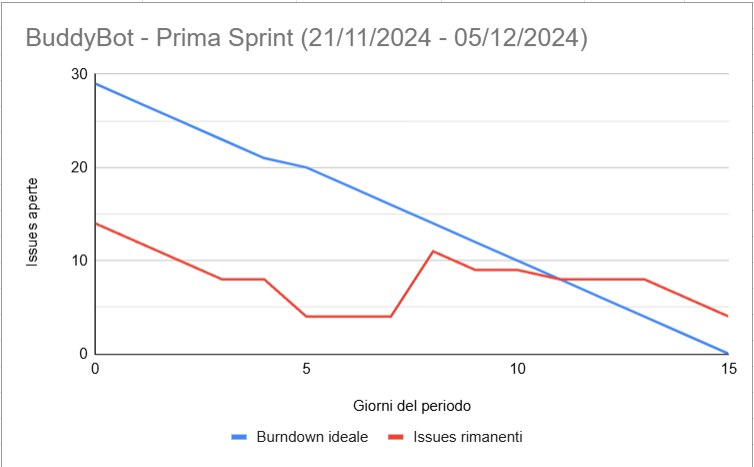
\includegraphics[width=\textwidth]{Primo periodo/Diagramma di Burndown - Primo periodo.jpg}
    \caption{Diagramma di Burndown del primo periodo} 
    \label{fig: Diagramma di Burndown del primo periodo}
\end{figure}
\newpage
\begin{figure}[h] 
    \centering
    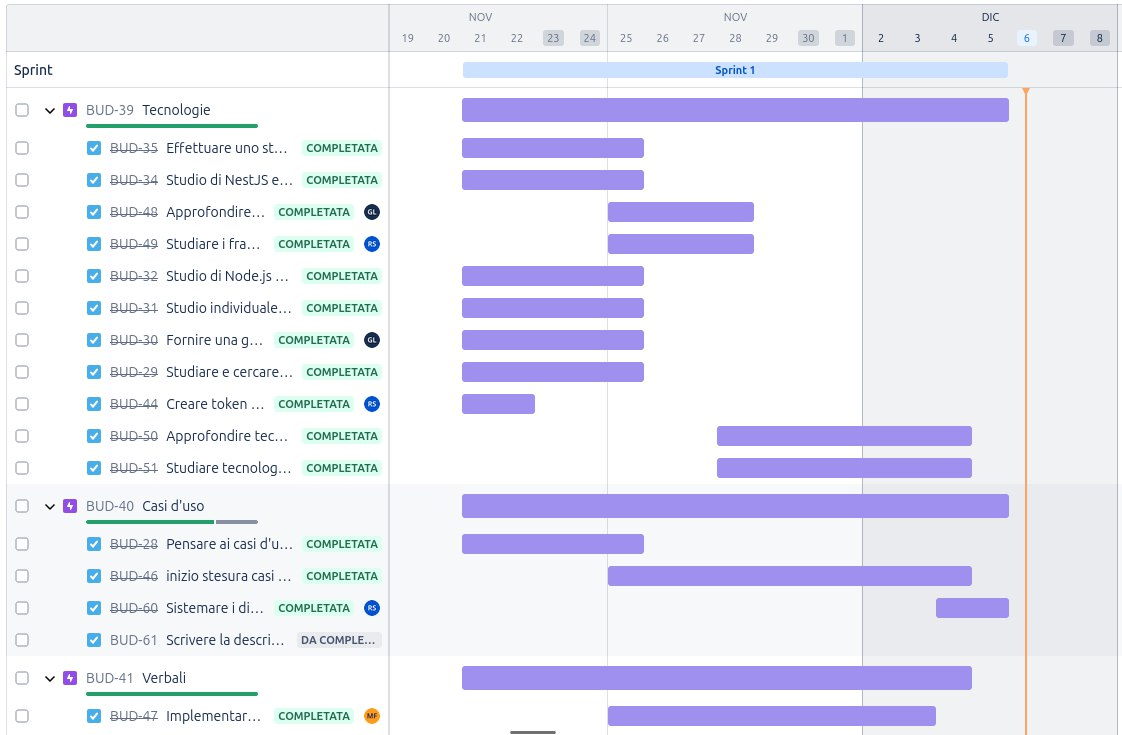
\includegraphics[width=\textwidth]{Primo periodo/Diagramma di Gantt (prima parte) - Primo periodo.jpg}
    \caption{Diagramma di Gantt primo periodo dal 21/11/2024 al 05/12/2024: prima parte} 
    \label{fig: Diagramma di Gantt primo periodo dal 21/11/2024 al 05/12/2024: prima parte}
\end{figure}
\newpage


\begin{figure}[h] 
    \centering
    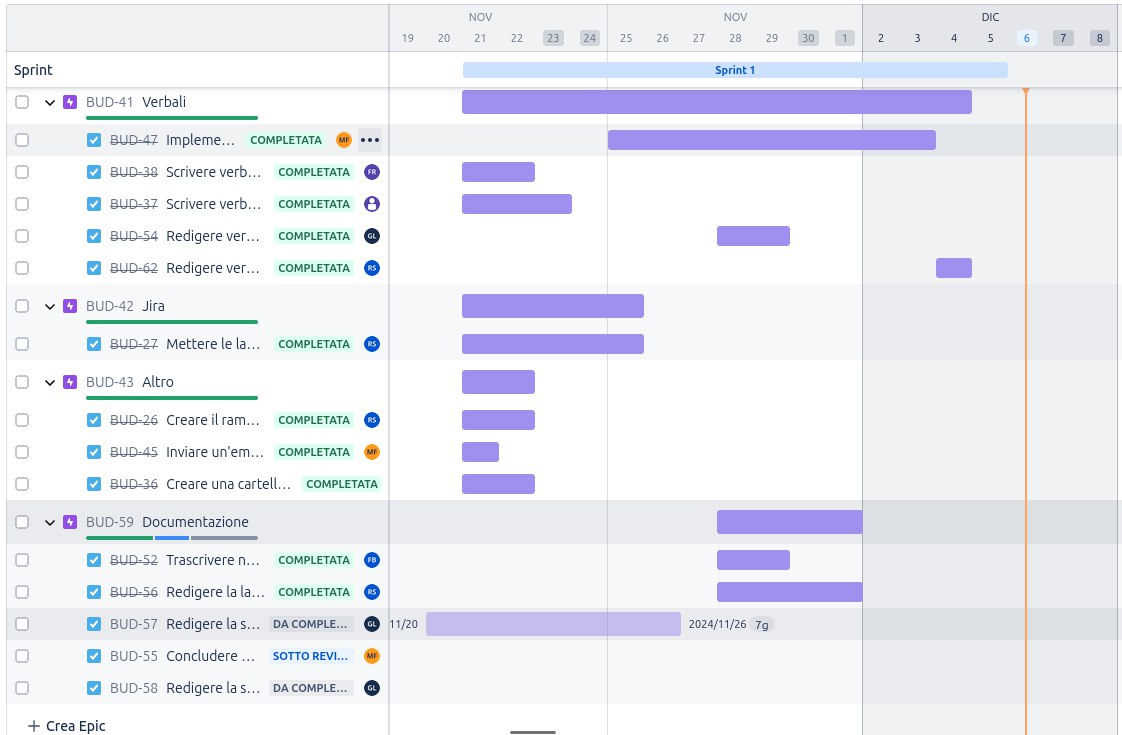
\includegraphics[width=\textwidth]{Primo periodo/Diagramma di Gantt (seconda parte) - Primo periodo.jpg}
    \caption{Diagramma di Gantt primo periodo dal 21/11/2024 al 05/12/2024: seconda parte} 
    \label{fig: Diagramma di Gantt primo periodo dal 21/11/2024 al 05/12/2024: seconda parte}
\end{figure}

\newpage
\subsubsubsection{Secondo periodo}
\label{sec:secondo periodo}
\begin{table}[h!]
    \centering
    \renewcommand{\arraystretch}{1.5} % Aumenta l'altezza delle righe
    \begin{tabularx}{\textwidth}{|X|X|}\hline
    \rowcolor[HTML]{FFD700} 
    \textbf{Data di inizio} & \textbf{Data di fine} \\ \hline
    06/12/2024 & 19/12/2024 \\ \hline
    \end{tabularx}
    \caption{Secondo periodo dedicato alla RTB}
\end{table}
Nel secondo periodo di lavoro, che va dal 6 dicembre al 19 dicembre 2024 e coincide con la seconda \textit{sprint}, abbiamo continuato a lavorare sull’\emph{Analisi dei casi d’uso}, identificando e documentando i punti chiave emersi sia nel confronto con il \emph{proponente} sia nel dialogo con il professor Cardin.\\
Abbiamo iniziato la trascrizione dei \emph{requisiti}, trasformando i \emph{casi d’uso} in specifiche tecniche e funzionali.\\
Per quanto riguarda le tecnologie, abbiamo confermato la nostra scelta e le abbiamo validate iniziando ad includerle nel \emph{PoC}\textsubscript{\textit{\textbf{G}}}, che rappresenta un primo prototipo. Il PoC, avviato durante questo sprint, risponde a domande riguardanti dati presenti su \emph{GitHub}\textsubscript{\textit{\textbf{G}}},
\emph{Confluence}\textsubscript{\textit{\textbf{G}}} e \emph{Jira}\textsubscript{\textit{\textbf{G}}}, presenta una struttura organizzata in classi e modulare, dispone di header che forniscono istruzioni all'\emph{LLM}\textsubscript{\textit{\textbf{G}}}, che saranno incrementati successivamente, e affronta alcune problematiche legate alla
ricerca di \emph{similarità}\textsubscript{\textit{\textbf{G}}} che saranno risolte con una migliore strutturazione dei dati. \\
Infine, abbiamo iniziato a compilare una lista di documenti di riferimento chiave e li abbiamo organizzati in \emph{Confluence}, \emph{Jira} e \emph{GitHub}, con l’obiettivo di garantire un contesto chiaro e accessibile per il chatbot.

\newpage
\begin{figure}[h] 
    \centering
    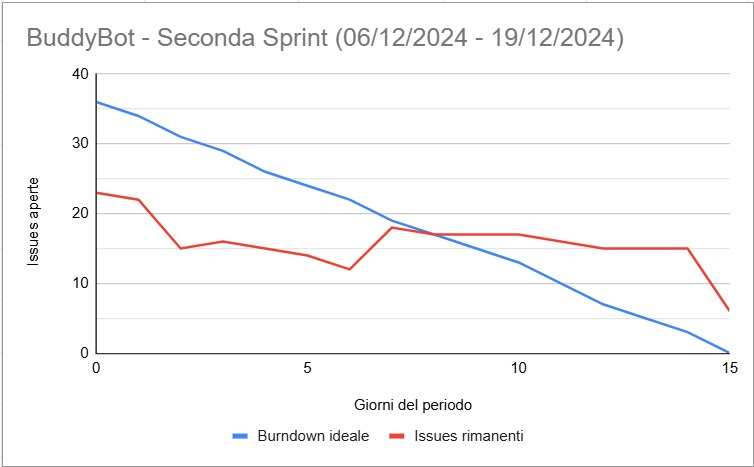
\includegraphics[width=\textwidth]{Secondo periodo/Diagramma di Burndown - Secondo periodo.jpg}
    \caption{Diagramma di Burndown del secondo periodo} 
    \label{fig: Diagramma di Burndown del secondo periodo}
\end{figure}

\newpage

\begin{figure}[h] 
    \centering
    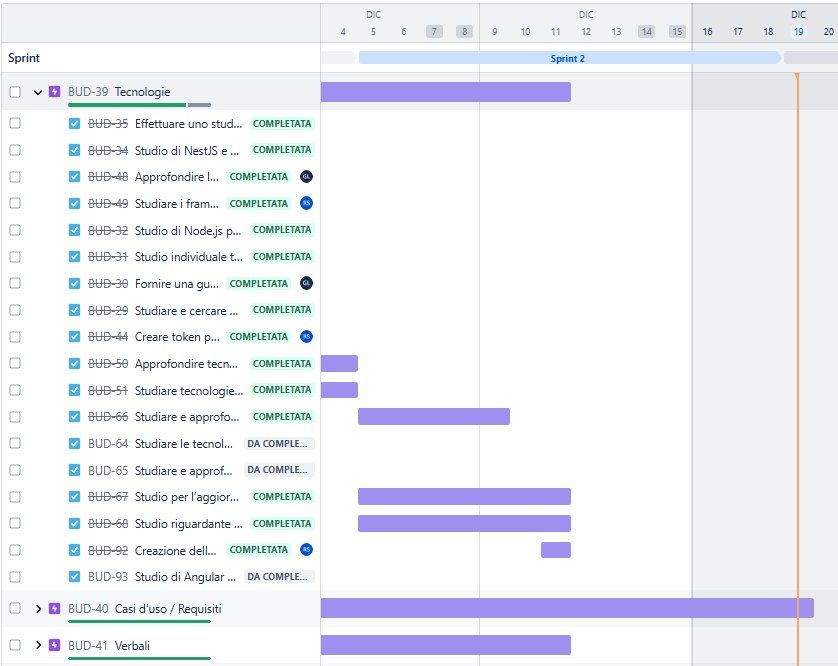
\includegraphics[width=\textwidth]{Secondo periodo/Diagramma di Gantt (prima parte) - Secondo periodo.jpg}
    \caption{Diagramma di Gantt secondo periodo dal 06/12/2024 - 19/12/2024: prima parte} 
    \label{fig: Diagramma di Gantt primo periodo dal 06/12/2024 - 19/12/2024: prima parte}
\end{figure}

\newpage

\begin{figure}[h] 
    \centering
    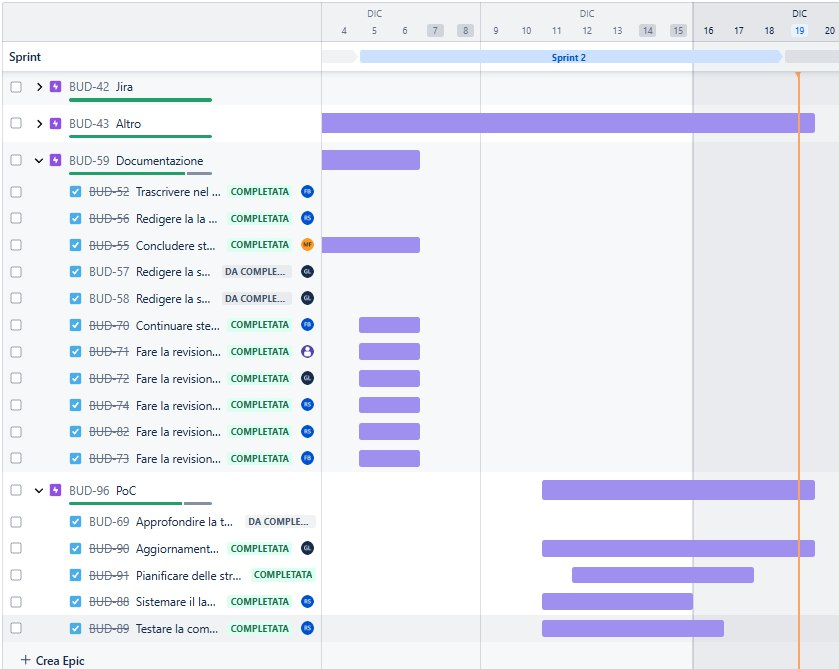
\includegraphics[width=\textwidth]{Secondo periodo/Diagramma di Gantt (seconda parte) - Secondo periodo.jpg}
    \caption{Diagramma di Gantt secondo periodo dal 06/12/2024 - 19/12/2024: seconda parte} 
    \label{fig: Diagramma di Gantt primo periodo dal 06/12/2024 - 19/12/2024: seconda parte}
\end{figure}

\newpage
\subsubsubsection{Terzo periodo}
\label{sec:terzo periodo}
\begin{table}[h!]
    \centering
    \renewcommand{\arraystretch}{1.5} % Aumenta l'altezza delle righe
    \begin{tabularx}{\textwidth}{|X|X|}\hline
    \rowcolor[HTML]{FFD700} 
    \textbf{Data di inizio} & \textbf{Data di fine} \\ \hline
    20/12/2024 & 03/01/2025 \\ \hline
    \end{tabularx}
    \caption{Terzo periodo dedicato alla RTB}
\end{table}
Nel terzo periodo di lavoro, che va dal 20 dicembre 2024 al 03 gennaio 2025 e coincide con la terza \textit{sprint}, abbiamo effettuato la revisione dei casi d’uso e dei requisiti, classificando i requisiti in obbligatori, desiderabili e opzionali, con particolare attenzione a quelli prioritari per il \emph{PoC}. 
Inoltre, abbiamo coinvolto il proponente per allineare le aspettative sui requisiti chiave e sugli obiettivi a breve termine, la definizione dei quali ci ha permesso di procedere con consapevolezza con lo studio delle tecnologie e con la programmazione.\\

\newpage
\begin{figure}[h] 
    \centering
    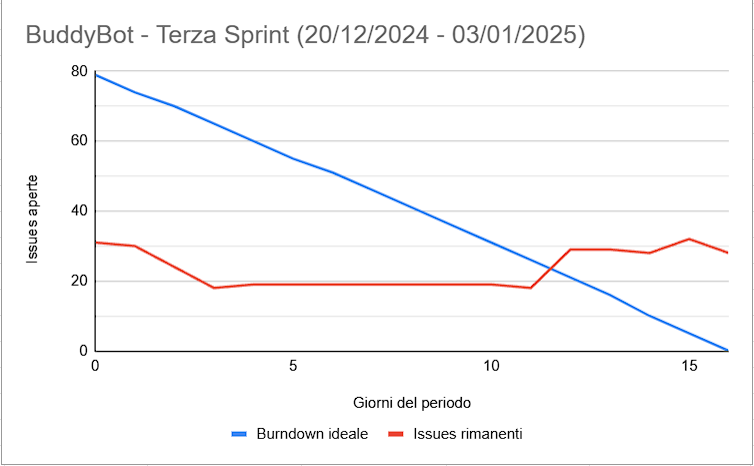
\includegraphics[width=\textwidth]{Terzo periodo/Diagramma di Burndown - Terzo periodo.png}
    \caption{Diagramma di Burndown del terzo periodo} 
    \label{fig: Diagramma di Burndown del terzo periodo}
\end{figure}

\newpage
\begin{figure}[h] 
    \centering
    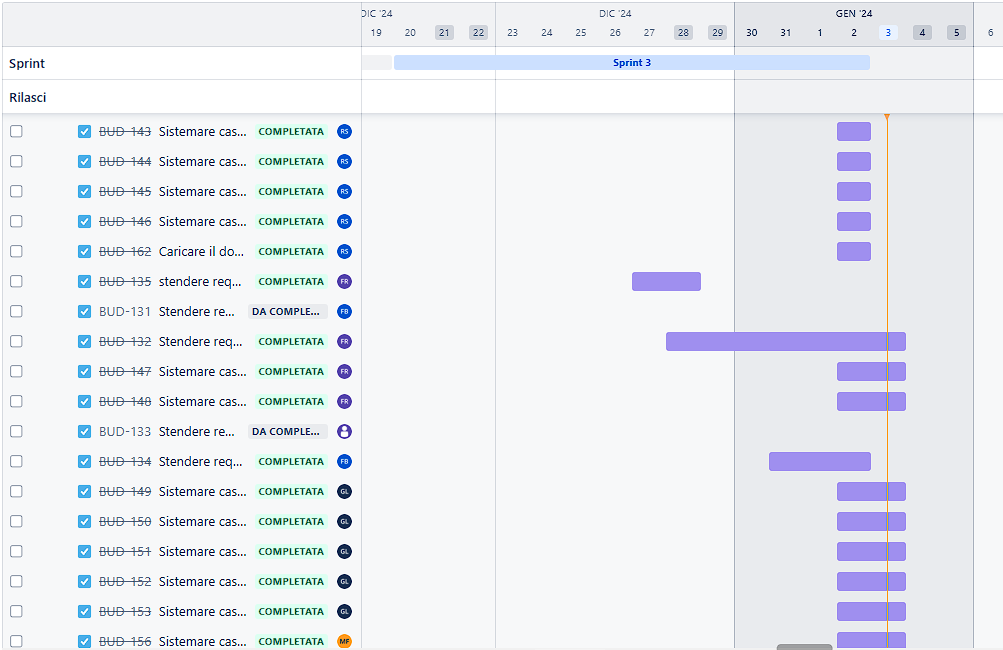
\includegraphics[width=\textwidth]{Terzo periodo/Diagramma di Gantt (prima parte) - Terzo periodo.png}
    \caption{Diagramma di Gantt terzo periodo dal 20/12/2024 - 03/01/2025: prima parte} 
    \label{fig: Diagramma di Gantt terzo periodo dal 20/12/2024 - 03/01/2025: prima parte}
\end{figure}

\newpage
\begin{figure}[h] 
    \centering
    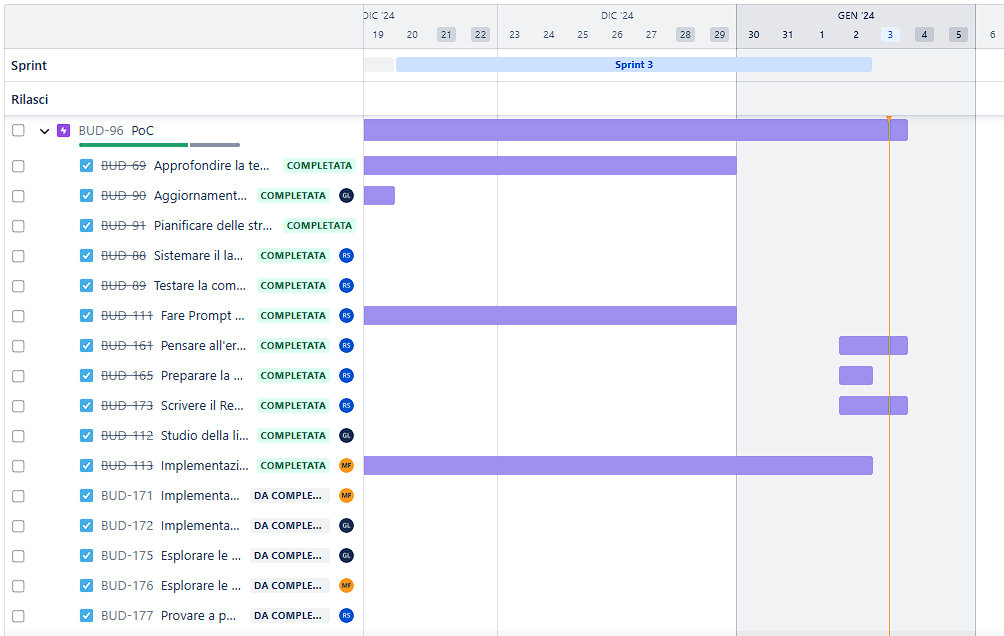
\includegraphics[width=\textwidth]{Terzo periodo/Diagramma di Gantt (seconda parte) - Terzo periodo.png}
    \caption{Diagramma di Gantt terzo periodo dal 20/12/2024 - 03/01/2025: seconda parte} 
    \label{fig: Diagramma di Gantt terzo periodo dal 20/12/2024 - 03/01/2025: seconda parte}
\end{figure}

\newpage
\subsubsubsection{Quarto periodo}
\label{sec:quarto periodo}
\begin{table}[h!]
    \centering
    \renewcommand{\arraystretch}{1.5} % Aumenta l'altezza delle righe
    \begin{tabularx}{\textwidth}{|X|X|}\hline
    \rowcolor[HTML]{FFD700} 
    \textbf{Data di inizio} & \textbf{Data di fine} \\ \hline
    04/01/2025 & 16/01/2025 \\ \hline
    \end{tabularx}
    \caption{Quarto periodo dedicato alla RTB}
\end{table}
Nel quarto periodo di lavoro, che si è svolto dal 4 gennaio 2025 al 16 gennaio 2025 e ha coinciso con la quarta \textit{sprint}, abbiamo portato a termine la redazione di alcuni documenti fondamentali per il progetto, tra cui: \emph{Analisi dei Requisiti}, \emph{Norme di Progetto} e \emph{Glossario}. 
Ci siamo promessi di completare i documenti del \emph{Piano di Progetto} e \emph{Piano di Qualifica} dopo la fine della sprint, in quanto avere disponibili anche i dati di quest'ultima risulta essenziale per ottenere una visione completa e dettagliata dell'avanzamento del lavoro e delle strategie di gestione della qualità.  
Parallelamente, abbiamo finalizzato il \emph{PoC}, dimostrando al proponente il lavoro svolto fino a questo momento. La presentazione ha permesso di verificare le scelte progettuali effettuate e di raccogliere eventuali feedback utili per migliorare ulteriormente il prodotto.
A seguito di un'attenta analisi del lavoro svolto e della verifica del rispetto degli obiettivi prefissati, abbiamo valutato di essere pronti per una consegna ufficiale in vista della \emph{RTB}.

\newpage
\begin{figure}[h] 
    \centering
    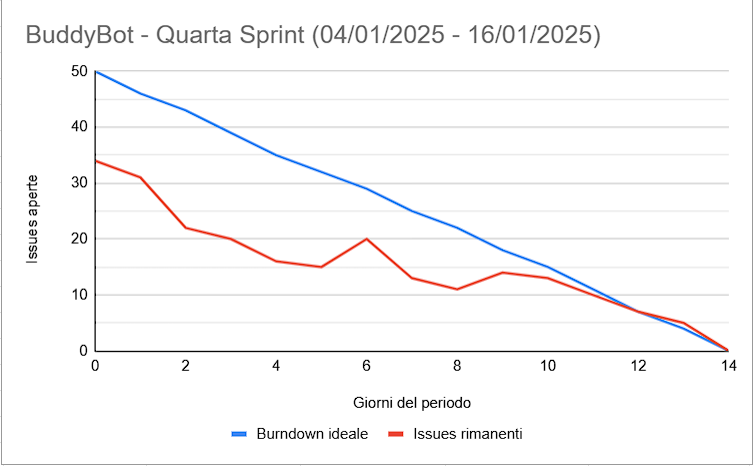
\includegraphics[width=\textwidth]{Quarto periodo/Diagramma di Burndown - Quarto periodo.png}
    \caption{Diagramma di Burndown del quarto periodo} 
    \label{fig: Diagramma di Burndown del quarto periodo}
\end{figure}

\newpage
\begin{figure}[h] 
    \centering
    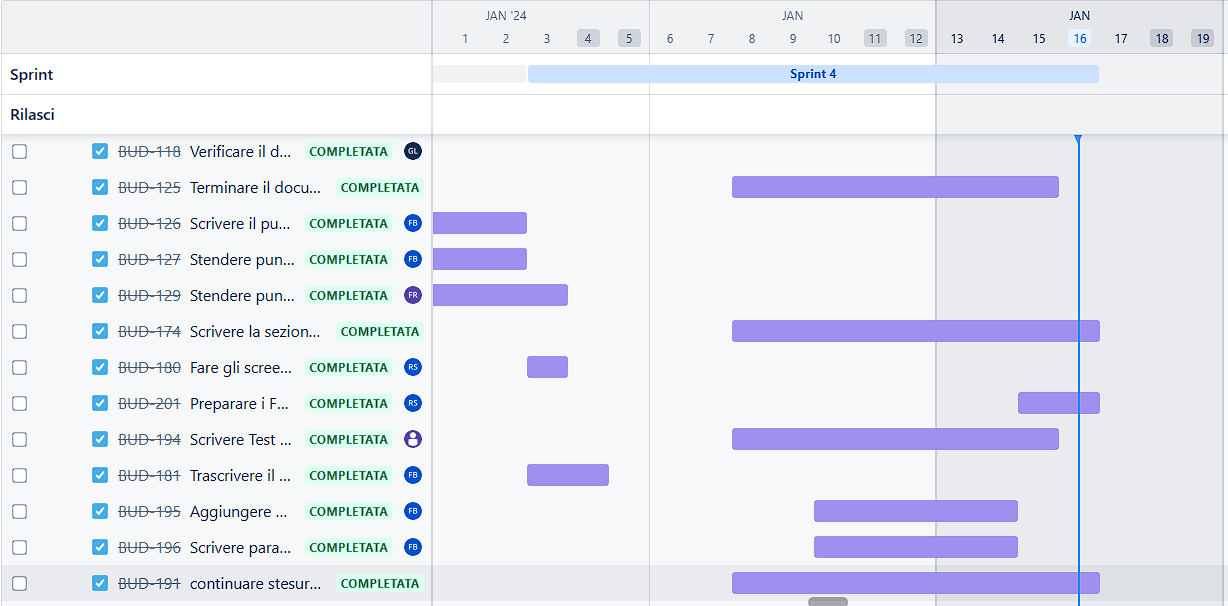
\includegraphics[width=\textwidth]{Quarto periodo/Diagramma di Gantt (prima parte) - Quarto periodo.png}
    \caption{Diagramma di Gantt del quarto periodo dal 04/01/2025 al 16/01/2025: prima parte} 
    \label{fig: Diagramma di Gantt quarto periodo dal 04/01/2025 al 16/01/2025: prima parte}
\end{figure}

\newpage
\begin{figure}[h] 
    \centering
    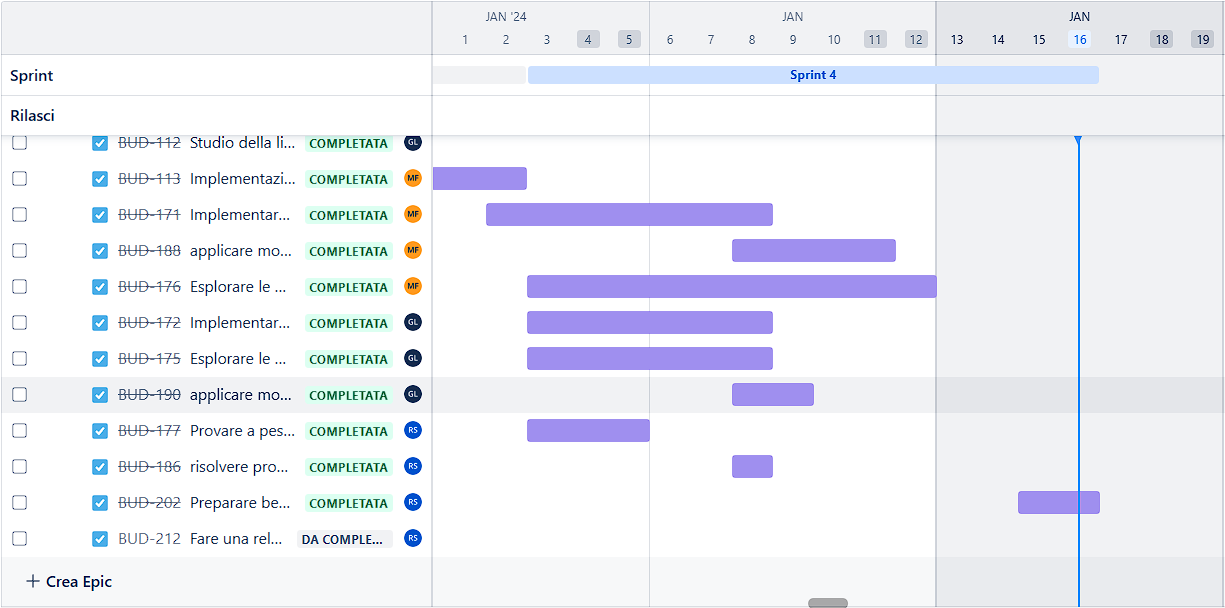
\includegraphics[width=\textwidth]{Quarto periodo/Diagramma di Gantt (seconda parte) - Quarto periodo.png}
    \caption{Diagramma di Gantt del quarto periodo dal 04/01/2025 al 16/01/2025: seconda parte} 
    \label{fig: Diagramma di Gantt quarto periodo dal 04/01/2025 al 16/01/2025 : seconda parte}
\end{figure}
\newpage

\subsection{Product Baseline}
\label{sec:product baseline}
\begin{table}[h!]
    \centering
    \renewcommand{\arraystretch}{1.5} % Aumenta l'altezza delle righe
    \begin{tabularx}{\textwidth}{|X|X|}\hline
    \rowcolor[HTML]{FFD700} 
    \textbf{Data di inizio} & \textbf{Data di fine} \\ \hline
    06/02/2025 & 03/04/2025 \\ \hline
    \end{tabularx}
    \caption{Periodo dello sviluppo della PB}
\end{table}
In questa fase del progetto, le {\emph{attività}}\textsubscript{\textit{\textbf{G}}} si concentrano sullo sviluppo del {\emph{Minimum Viable Product (MVP)}}\textsubscript{\textit{\textbf{G}}}. 
Il processo inizia con una fase di progettazione, che prevede un’analisi approfondita per identificare i componenti principali dell’applicazione e le loro interconnessioni, così da poter definire un’architettura solida. 
Successivamente, si procede con la programmazione, implementando i requisiti e i casi d’uso concordati con il \emph{proponente} sotto forma di codice. 
Parallelamente, viene redatta la documentazione, che comprende la {\emph{Specifica Tecnica}}\textsubscript{\textit{\textbf{G}}} e il {\emph{Manuale Utente}}\textsubscript{\textit{\textbf{G}}}.\\
Le fasi principali del \emph{Product Baseline} saranno suddivise come segue:
\begin{itemize}
\item \textbf{Analisi preliminare della progettazione}: il team condurrà uno studio iniziale sulla progettazione e sui \emph{design pattern}\textsubscript{\textit{\textbf{G}}}, con l’obiettivo di individuare l’architettura più adatta al software in sviluppo;
\item \textbf{Progettazione logica}: in questa fase si definirà una visione generale dell’architettura del prodotto, basandosi sull’Analisi dei Requisiti. Verranno identificate le componenti principali, le loro funzionalità essenziali e le relazioni tra di esse;
\item \textbf{Progettazione di dettaglio}: una volta stabilita l’architettura di alto livello, si procederà a una definizione più approfondita, descrivendo in dettaglio le unità architetturali, le loro funzionalità e le dipendenze reciproche;
\item \textbf{Sviluppo del Minimum Viable Product}: in questa fase si procederà con la scrittura del codice dell’ \emph{MVP}, seguendo l’architettura definita e implementando tutte le funzionalità individuate;
\item \textbf{Redazione e aggiornamento della documentazione}: questa attività sarà svolta parallelamente alle altre fasi, garantendo che il lavoro sia adeguatamente documentato per il team attuale, gli sviluppatori futuri e l’utente finale.
\end{itemize}

\subsubsection{Attività}

\begin{itemize}
\item \textbf{\emph{Norme di Progetto}}: aggiornamento del documento con l’aggiunta di eventuali nuove tecnologie e strumenti utilizzati, o cambiamenti nel proprio {\emph{Way of Working}}\textsubscript{\textit{\textbf{G}}};
\item \textbf{\emph{Piano di Progetto}}: ristrutturazione del documento seguendo il feedback ricevuto dalla revisione {\emph{RTB}}\textsubscript{\textit{\textbf{G}}}, e aggiornamento continuativo dello stato del progetto nei vari periodi della {\emph{PB}}\textsubscript{\textit{\textbf{G}}};
\item \textbf{\emph{Piano di Qualifica}}: ampliamento della sezione "\emph{Cruscotto di valutazione}" all’interno del documento seguendo il feedback ricevuto dalla revisione \emph{RTB}, aggiunta dei test di integrazione e di unità;
\item \textbf{\emph{Analisi dei Requisiti}}: aggiunta di maggior dettaglio nella modellazione dei \emph{casi d’uso} e nella descrizione delle funzionalità;
\item \textbf{\emph{Glossario}}: aggiornamento del documento con nuovi termini incontrati nel periodo \emph{PB};
\item \textbf{\emph{Specifica Tecnica}}: la \emph{Specifica Tecnica} ha lo scopo di servire da linea guida per gli sviluppatori che andranno ad estendere o mantenere il prodotto. Il team \emph{SWEg Labs} vi inserirà tutte le informazioni riguardanti i linguaggi e le tecnologie utilizzate, l’architettura del sistema e le scelte progettuali effettuate per il prodotto;
\item \textbf{\emph{Manuale Utente}}: il \emph{Manuale Utente} ha lo scopo di illustrare le istruzioni per l’utilizzo e le funzionalità fornite dall’applicativo. L’utente sarà quindi a conoscenza dei requisiti minimi necessari per il corretto funzionamento dello stesso, di come installarlo in locale e di come farne un utilizzo consapevole;
\item \textbf{\emph{Scrittura del codice}}: attività di codifica seguendo l’architettura definita;
\item \textbf{\emph{Glossario}}: attività di verifica, svolta in parallelo alla codifica.
\end{itemize}


\subsubsection{Periodi}
\label{sec:periodi_PB}

\subsubsubsection{Quinto periodo}
\label{sec:quinto periodo}
\begin{table}[h!]
    \centering
    \renewcommand{\arraystretch}{1.5} % Aumenta l'altezza delle righe
    \begin{tabularx}{\textwidth}{|X|X|}\hline
    \rowcolor[HTML]{FFD700} 
    \textbf{Data di inizio} & \textbf{Data di fine} \\ \hline
    06/02/2025 & 20/02/2025 \\ \hline
    \end{tabularx}
    \caption{Quinto periodo dedicato alla PB}
\end{table}
Il quinto periodo che va dal 6 al 20 febbraio 2025, abbiamo compiuto alcune sistemazioni all'\emph{Analisi dei Requisiti}, seguendo i
consigli del professor Cardin. Abbiamo inoltre incominciato la progettazione, in particolare concentrandoci sulle seguenti funzionalità:
\begin{itemize}
    \item Generazione di una risposta;
    \item Aggiornamento automatico del {\emph{database vettoriale}}\textsubscript{\textit{\textbf{G}}};
    \item Inizializzazione, refresh e scroll dell'interfaccia grafica;
    \item Rendering grafico di domanda e risposta;
    \item Aggiornamento del badge di segnalazione dell'esito dell'aggiornamento del database vettoriale;
    \item Salvataggio dei messaggi nello storico;
    \item Recupero dei messaggi dallo storico;
    \item Generazione di domande per proseguire la conversazione.
\end{itemize}
Abbiamo avviato la scrittura della \emph{Specifica Tecnica} e del \emph{Manuale Utente}, focalizzandoci sulla sezione
"\emph{Cosa chiedere e come chiederlo}".
Dal punto di vista architetturale, abbiamo deciso di adottare l’{\emph{architettura esagonale}}\textsubscript{\textit{\textbf{G}}}
per garantire maggiore modularità e manutenibilità del sistema.

\newpage
\begin{figure}[h] 
    \centering
    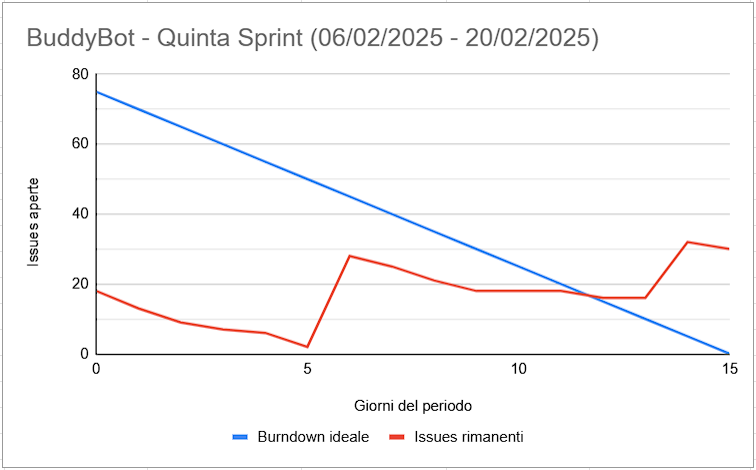
\includegraphics[width=\textwidth]{Quinto periodo/Diagramma di Burndown - Quinto periodo.png}
    \caption{Diagramma di Burndown del quinto periodo} 
    \label{fig: Diagramma di Burndown del quinto periodo}
\end{figure}
\newpage
\begin{figure}[h] 
    \centering
    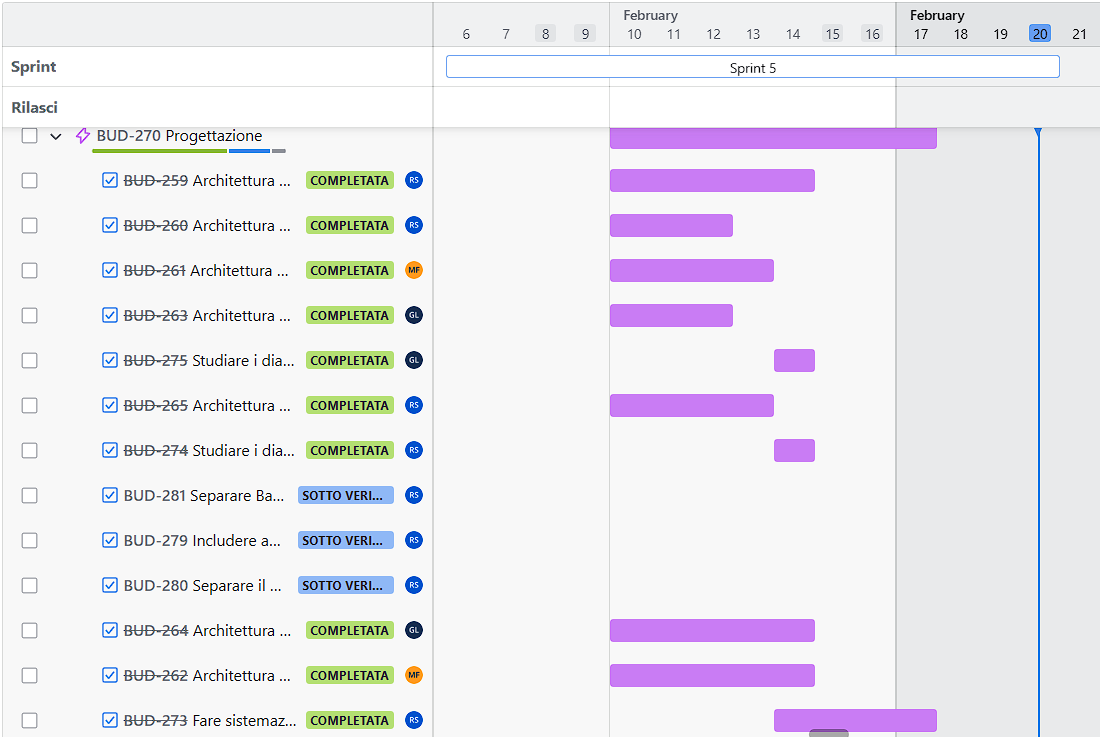
\includegraphics[width=\textwidth]{Quinto periodo/Diagramma di Gantt (prima parte) - Quinto periodo.png}
    \caption{Diagramma di Gantt quinto periodo dal 06/02/2024 al 20/02/2025: prima parte} 
    \label{fig: Diagramma di Gantt quinto periodo dal 06/02/2024 al 20/02/2025: prima parte}
\end{figure}
\newpage
\begin{figure}[h] 
    \centering
    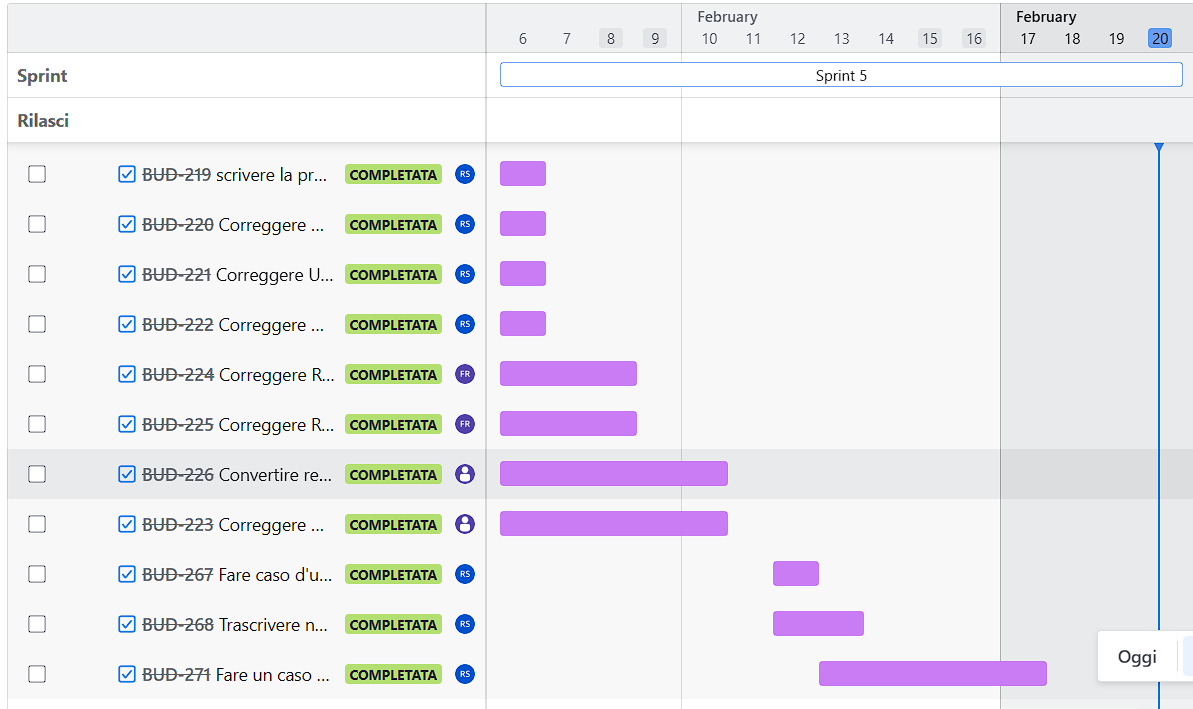
\includegraphics[width=\textwidth]{Quinto periodo/Diagramma di Gantt (seconda parte) - Quinto periodo.png}
    \caption{Diagramma di Gantt quinto periodo dal 06/02/2024 al 20/02/2025: seconda parte} 
    \label{fig: Diagramma di Gantt quinto periodo dal 06/02/2024 al 20/02/2025: seconda parte}
\end{figure}

\newpage


\subsubsubsection{Sesto periodo}
\label{sec:sesto periodo}
\begin{table}[h!]
    \centering
    \renewcommand{\arraystretch}{1.5} % Aumenta l'altezza delle righe
    \begin{tabularx}{\textwidth}{|X|X|}\hline
    \rowcolor[HTML]{FFD700} 
    \textbf{Data di inizio} & \textbf{Data di fine} \\ \hline
    21/02/2025 & 06/03/2025 \\ \hline
    \end{tabularx}
    \caption{Sesto periodo dedicato alla PB}
\end{table}
Il sesto periodo, che va dal 21 febbraio al 6 marzo 2025, è stato dedicato a diverse attività fondamentali per il progresso del progetto.\\
Abbiamo corretto i diagrammi di progettazione affinché rispettassero con precisione le esigenze del \emph{proponente} e trasposto i diagrammi del \emph{backend} dell'applicazione in codice \emph{Python}. Inoltre, ci siamo occupati dello sviluppo dei \emph{test di integrazione}\textsubscript{\textbf{\textit{G}}} e abbiamo condotto alcuni esperimenti grafici per il frontend in \emph{Angular}.
Infine, abbiamo iniziato a lavorare all'ottimizzazione della gestione delle modifiche e delle eliminazioni dei documenti nell'aggiornamento automatico del \emph{database vettoriale}, per migliorarne l'\emph{efficienza} e l'affidabilità.

\newpage
\begin{figure}[h] 
    \centering
    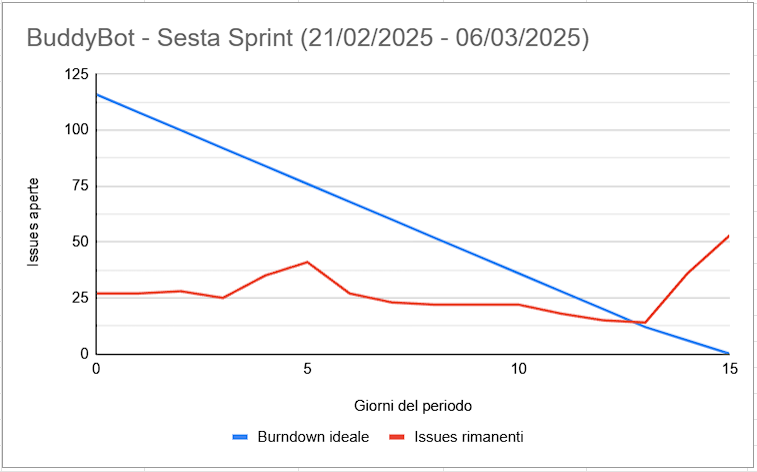
\includegraphics[width=\textwidth]{Sesto periodo/Diagramma di Burndown - Sesto periodo.png}
    \caption{Diagramma di Burndown del sesto periodo} 
    \label{fig: Diagramma di Burndown del sesto periodo}
\end{figure}
\newpage
\begin{figure}[h] 
    \centering
    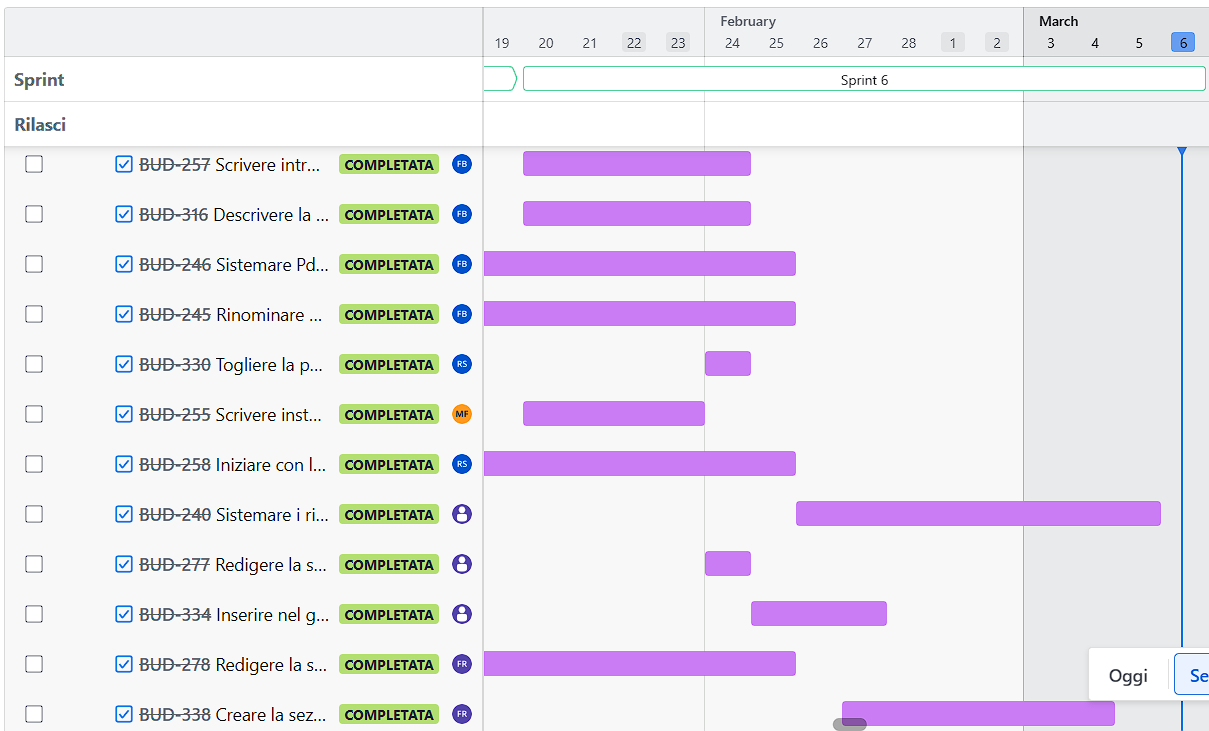
\includegraphics[width=\textwidth]{Sesto periodo/Diagramma di Gantt (prima parte) - Sesto periodo.png}
    \caption{Diagramma di Gantt sesto periodo dal 21/02/2025 - 06/03/2025: prima parte} 
    \label{fig: Diagramma di Gantt sesto periodo dal 21/02/2025 - 06/03/2025: prima parte}
\end{figure}
\newpage
\begin{figure}[h] 
    \centering
    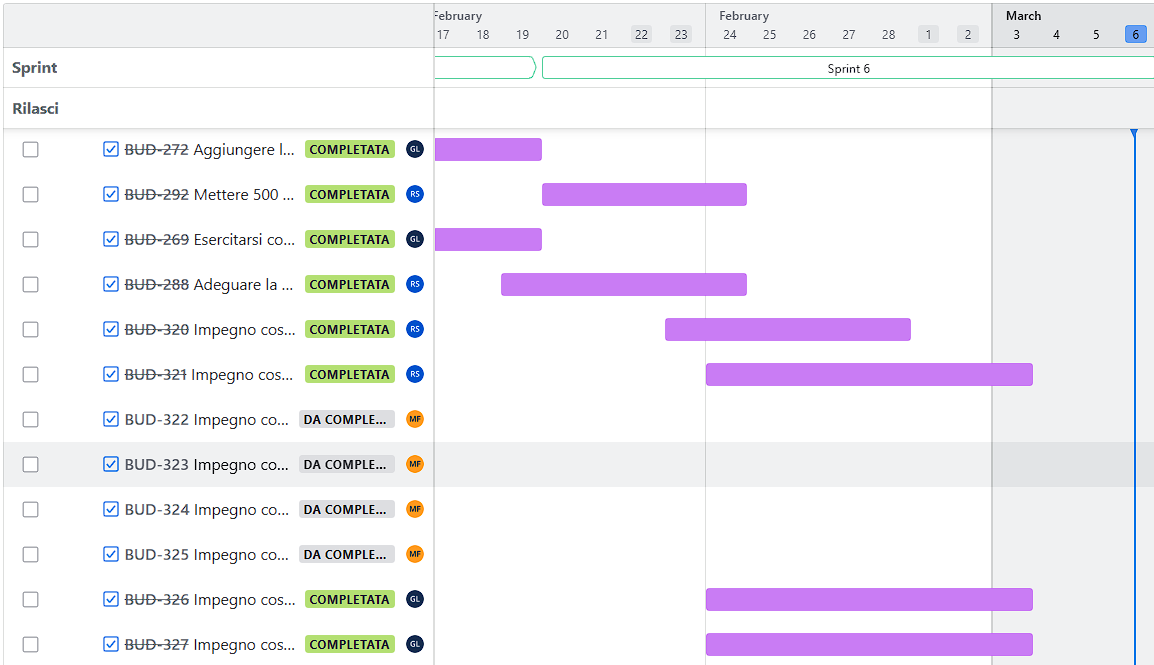
\includegraphics[width=\textwidth]{Sesto periodo/Diagramma di Gantt (seconda parte) - Sesto periodo.png}
    \caption{Diagramma di Gantt sesto periodo dal 21/02/2025 - 06/03/2025: seconda parte} 
    \label{fig: Diagramma di Gantt sesto periodo dal 21/02/2025 - 06/03/2025: seconda parte}
\end{figure}

\newpage


\subsubsubsection{Settimo periodo}
\label{sec:settimo periodo}
\begin{table}[h!]
    \centering
    \renewcommand{\arraystretch}{1.5} % Aumenta l'altezza delle righe
    \begin{tabularx}{\textwidth}{|X|X|}\hline
    \rowcolor[HTML]{FFD700} 
    \textbf{Data di inizio} & \textbf{Data di fine} \\ \hline
    07/03/2025 & 19/03/2025 \\ \hline
    \end{tabularx}
    \caption{Settimo periodo dedicato alla PB}
\end{table}
Il settimo periodo, che va dal 7 al 19 marzo 2025, è stato dedicato principalmente alla programmazione dell'\emph{MVP}.\\
In particolare, sono state implementate le seguenti funzionalità:
\begin{itemize}
    \item L'ottimizzazione della gestione delle modifiche e delle eliminazioni dei documenti nell'aggiornamento automatico del \emph{database vettoriale}, che, in particolare, è stata implementata differenziando la gestione tra l'aggiornamento dei file di \emph{GitHub}\textsubscript{\textbf{\textit{G}}} e l'aggiornamento degli altri documenti;
    \item L'implementazione di un sistema di \emph{logging}\textsubscript{\textbf{\textit{G}}} per l'aggiornamento automatico, in particolare prevedendo la scrittura in due file: un file txt dedicato ai log consuntivi di fine aggiornamento e un file cron.log dedicato ai log istantanei stampati durante l'esecuzione dello \emph{script}\textsubscript{\textbf{\textit{G}}} di aggiornamento da parte del \emph{cron}\textsubscript{\textbf{\textit{G}}};
    \item Il completamento del \emph{frontend} del prodotto, in particolare l'implementazione della visualizzazione dello storico dei messaggi e del corrispondente scroll infinito, della visualizzazione dei link correlati alle risposte e della gestione degli errori mediante segnali di avviso temporizzati.
\end{itemize}
A corredo di ciò, abbiamo proceduto a trascrivere tutti i diagrammi della progettazione nel documento di \emph{Specifica Tecnica} e a redigere la guida all'utilizzo del prodotto nel \emph{Manuale Utente}.\\
Infine, il giorno mercoledì 19 marzo, al termine del periodo, abbiamo svolto la \emph{demo}\textsubscript{\textbf{\textit{G}}} dell'\emph{MVP} assieme al \emph{proponente}, che ha validato il lavoro svolto, consentendo quindi al team di considerare conclusa l'attività di programmazione.

\newpage
\begin{figure}[h] 
    \centering
    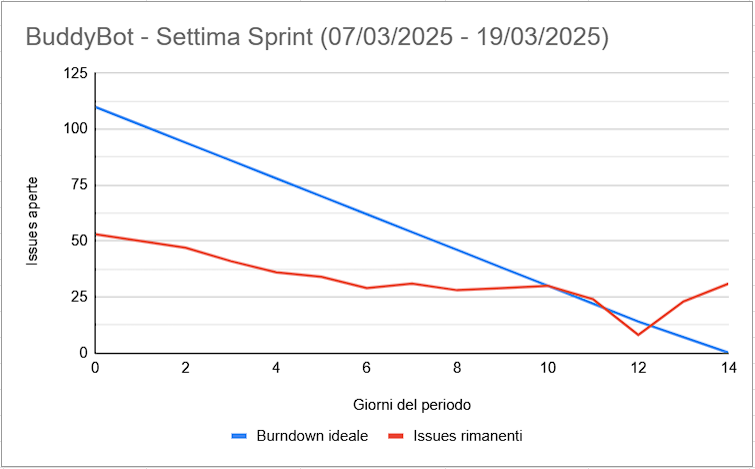
\includegraphics[width=\textwidth]{Settimo periodo/Diagramma di Burndown - Settimo periodo.png}
    \caption{Diagramma di Burndown del settimo periodo} 
    \label{fig: Diagramma di Burndown del settimo periodo}
\end{figure}
\newpage
\begin{figure}[h] 
    \centering
    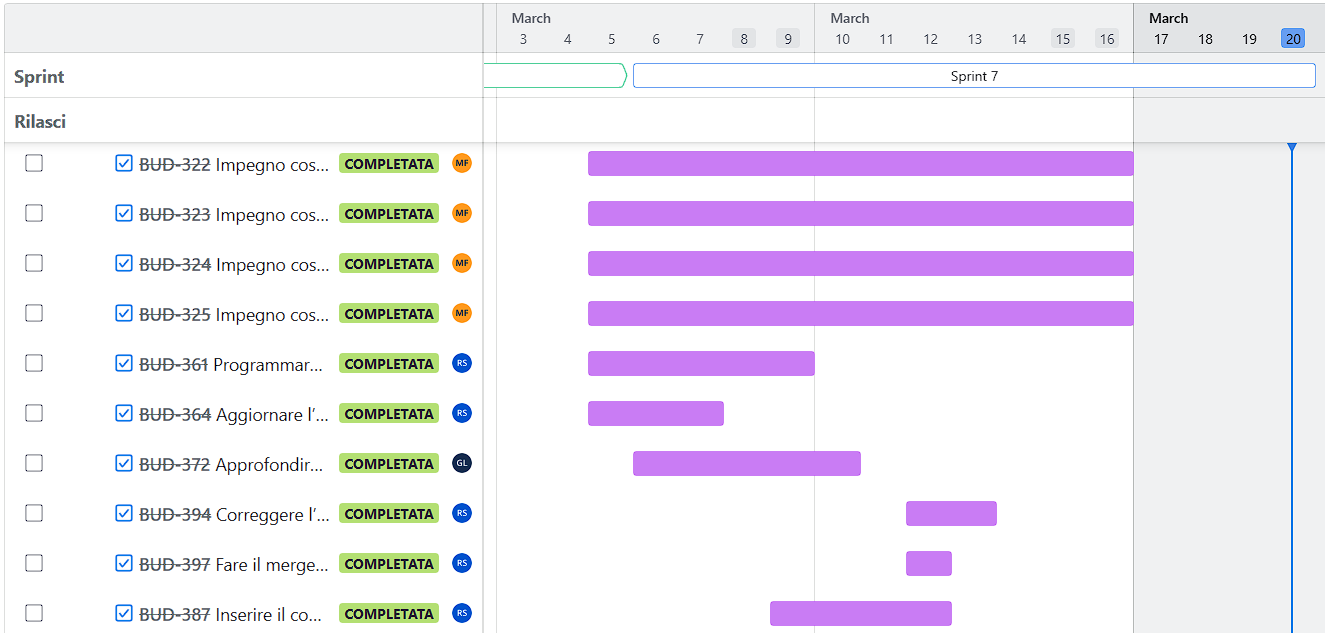
\includegraphics[width=\textwidth]{Settimo periodo/Diagramma di Gantt (prima parte) - Settimo periodo.png}
    \caption{Diagramma di Gantt settimo periodo dal 07/03/2025 - 19/03/2025: prima parte} 
    \label{fig: Diagramma di Gantt settimo periodo dal 07/03/2025 - 19/03/2025: prima parte}
\end{figure}
\newpage
\begin{figure}[h] 
    \centering
    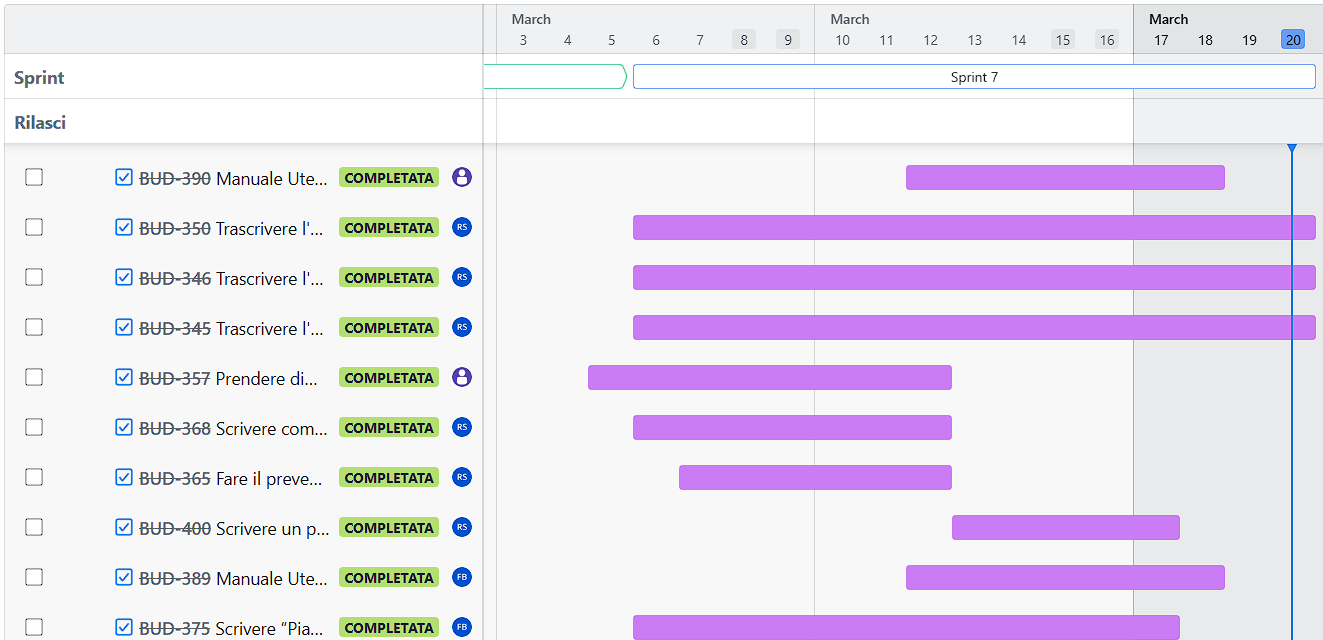
\includegraphics[width=\textwidth]{Settimo periodo/Diagramma di Gantt (seconda parte) - Settimo periodo.png}
    \caption{Diagramma di Gantt settimo periodo dal 07/03/2025 - 19/03/2025: seconda parte} 
    \label{fig: Diagramma di Gantt settimo periodo dal 07/03/2025 - 19/03/2025: seconda parte}
\end{figure}

\newpage
\subsubsubsection{Ottavo periodo}
\label{sec:ottavo periodo}
\begin{table}[h!]
    \centering
    \renewcommand{\arraystretch}{1.5} % Aumenta l'altezza delle righe
    \begin{tabularx}{\textwidth}{|X|X|}\hline
    \rowcolor[HTML]{FFD700} 
    \textbf{Data di inizio} & \textbf{Data di fine} \\ \hline
    20/03/2025 & 03/04/2025 \\ \hline
    \end{tabularx}
    \caption{Ottavo periodo dedicato alla PB}
\end{table}
L'ottavo periodo, che va dal 20 marzo al 3 aprile 2025, è stato dedicato alla finalizzazione e revisione del progetto. Gli obiettivi fissati per l'ottavo periodo includevano l'aggiornamento e il completamento della documentazione, oltre alla comunicazione con il professor Cardin per schedulare l'incontro di revisione \emph{Product Baseline}, fissato infine il giorno 3 aprile.\\
Tra le principali attività, si è proceduto con l'aggiornamento del cruscotto di valutazione della qualità nel \emph{Piano di Qualifica}, l'inserimento delle immagini definitive dei diagrammi di \emph{progettazione} nella \emph{Specifica Tecnica}, la scrittura della lettera di presentazione, e la rilettura e la verifica di tutti i documenti per correggere errori e migliorare la loro coerenza. Inoltre, è stato sistemato il README del \emph{repository} dell’\emph{MVP} su richiesta del \emph{proponente}, ed è stata redatta la presentazione per l’incontro con il professor Cardin.

\newpage
\begin{figure}[h] 
    \centering
    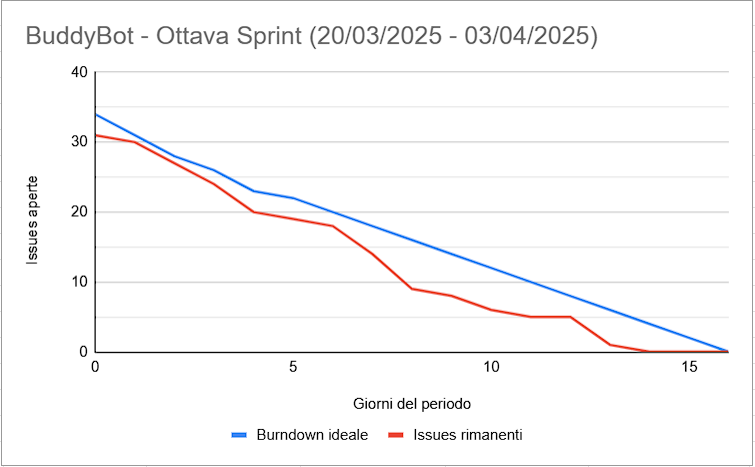
\includegraphics[width=\textwidth]{Ottavo periodo/Diagramma di Burndown - Ottavo periodo.png}
    \caption{Diagramma di Burndown dell'ottavo periodo} 
    \label{fig: Diagramma di Burndown dell'ottavo periodo}
\end{figure}
\newpage
\begin{figure}[h] 
    \centering
    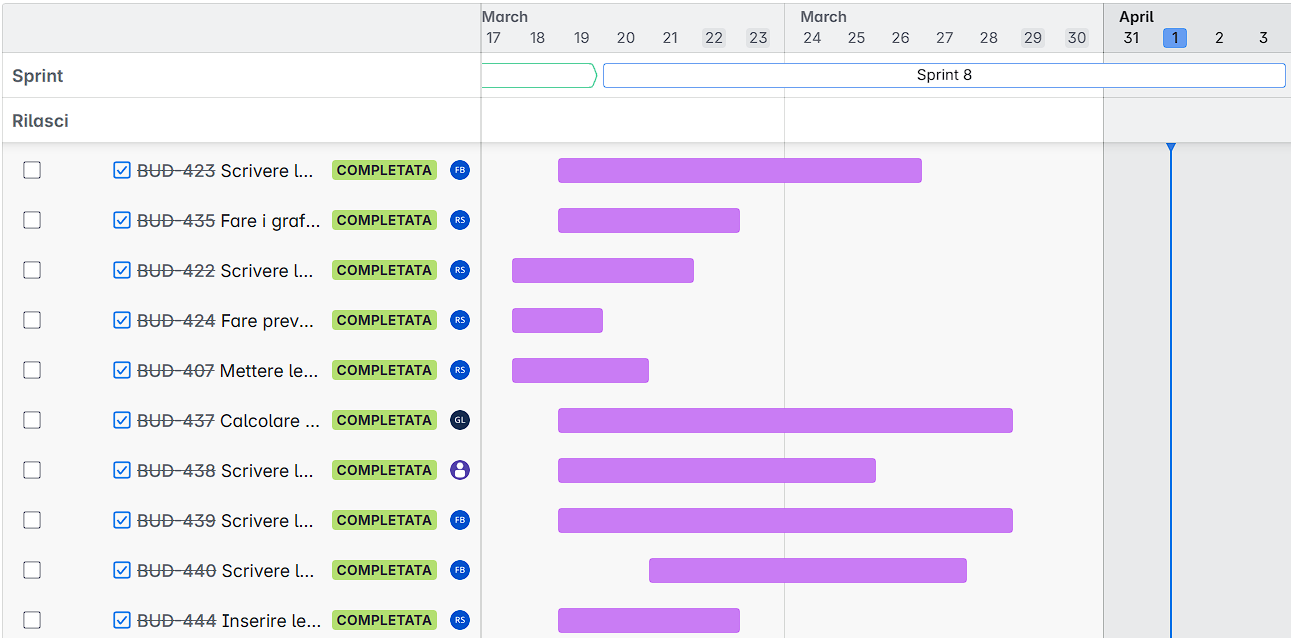
\includegraphics[width=\textwidth]{Ottavo periodo/Diagramma di Gantt (prima parte) - Ottavo periodo.png}
    \caption{Diagramma di Gantt ottavo periodo dal 20/03/2025 - 03/04/2025: prima parte} 
    \label{fig: Diagramma di Gantt ottavo periodo dal 20/03/2025 - 03/04/2025: prima parte}
\end{figure}
\newpage
\begin{figure}[h] 
    \centering
    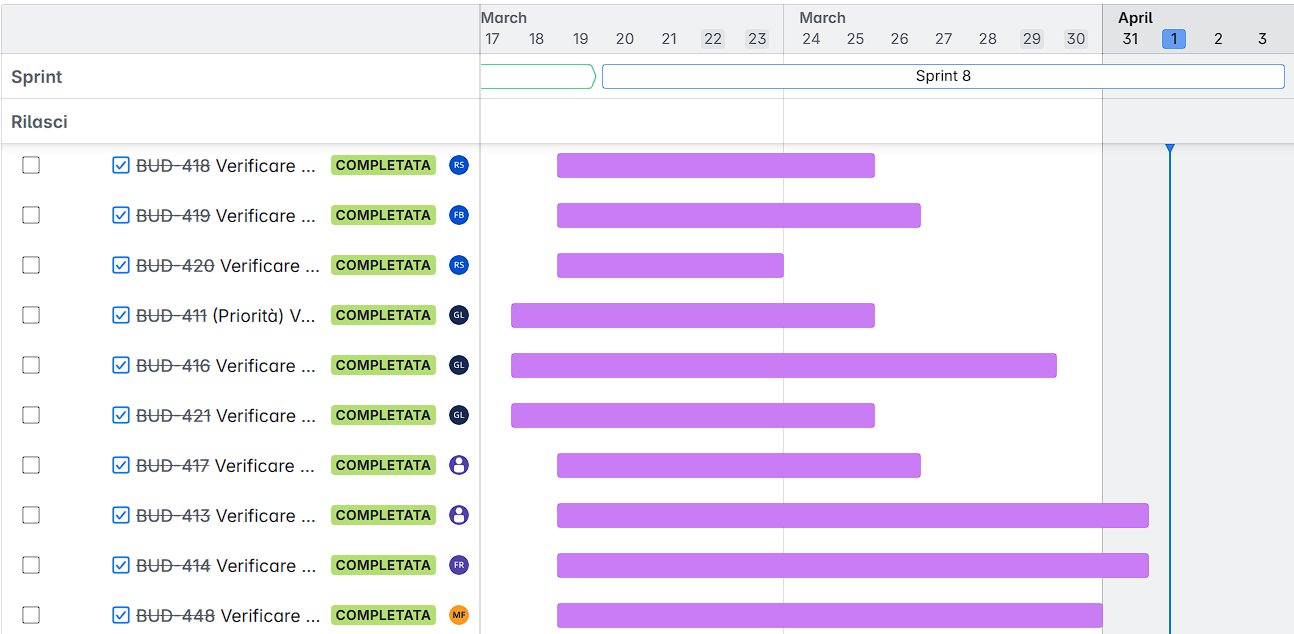
\includegraphics[width=\textwidth]{Ottavo periodo/Diagramma di Gantt (seconda parte) - Ottavo periodo.png}
    \caption{Diagramma di Gantt ottavo periodo dal 20/03/2025 - 03/04/2025: seconda parte} 
    \label{fig: Diagramma di Gantt ottavo periodo dal 20/03/2025 - 03/04/2025: seconda parte}
\end{figure}
\newpage

